\section{Lösungskonzept} \label{solution-concept}
Dieses Kapitel soll aufzeigen mit welcher konkreten Ausprägung der Blockchain Techologie der gewählte Use-Case realisiert werden kann. Dazu wird im ersten Schritt eine SWOT-Analyse zur Blockchain Technologie allgemein durchgeführt und die Ergebnise beschrieben. In Schritt zwei kommt eine Nutzwertanalyse zum Einsatz anhand welcher ermittelt wird welche Ausprägung der Technologie sich zur Umsetzung bestmöglichst eignet.

\subsection{SWOT-Analyse der \textit{Blockchain-Technologie}} \label{swot-analyse}
Durch die Vielzahl an unterschiedlichen Use-Cases die mittels der Blockchain Technologie umgesetzt werden ist es nötig für den spezifischen Use-Case der Chargenrückverfolgung die Technologie einer SWOT-Analyse zu unterziehen. Hierdurch wird gewährleistet, dass die Technologie für den Use-Case überhaupt geeignet ist. Im folgenden werden daher aus interner Sicht die Stärken und Schwächen gegenübergestellt, sowie die dadurch möglichen externen Chancen und Risiken diskutiert. Abbildung \ref{fig:blockchain-technology-swot-analysis} zeigt eine schematische Sicht der SWOT-Analyse.

\begin{figure}[H]
	\centering
	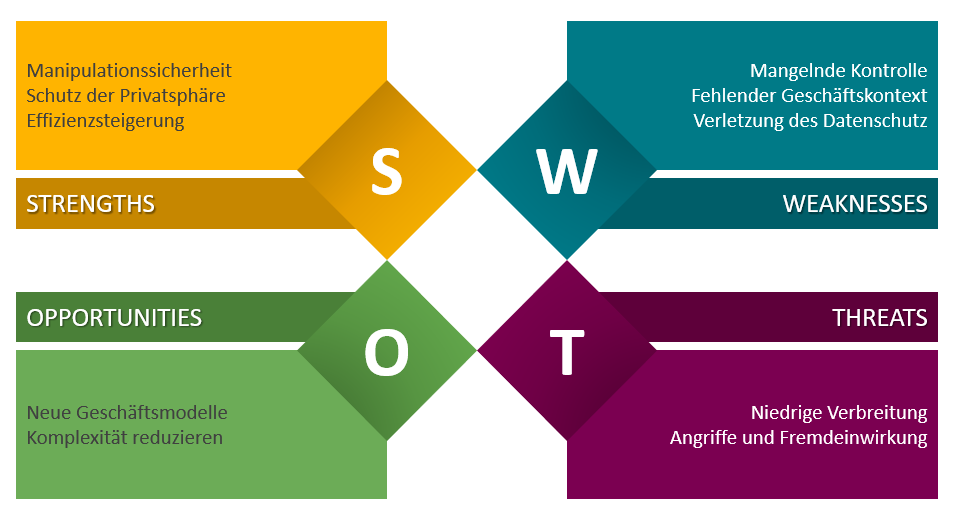
\includegraphics[width=1\linewidth]{pictures/blockchain-technology-swot-analysis}
	\caption[Blockchain Technologie SWOT Analyse]{Blockchain Technologie SWOT Analyse (eigene Darstellung)}
	\label{fig:blockchain-technology-swot-analysis}
\end{figure}

\subsubsection{Stärken}
\paragraph{Manipulationsicherheit}
Eine der Schlüsselstärken der Technologie ist, dass sie eine Manipulation von Datensätzen direkt erkennbar macht durch die Art und Weise wie Transaktionen gespeichert und verknüpft werden.

\paragraph{Schutz der Privatsphäre}
Durch eine Implementierung eines Berechtigungskonzepts können Teilnehmer des Netzwerks eigenständig definieren wer auf die Daten zugreifen kann, für welchen Zweck und für welchen Zeitraum. Diese Regeln werden in Smart Contracts programmatisch abgebildet und bei jeder Ausführung geprüft. So lassen sich beispielsweise komplexe Berechtigungsstrukturen direkt innerhalb des Netzwerks abbilden ohne dazu eine zusätzliche Abstraktionsebene einführen zu müssen. 

\paragraph{Effizienzsteigerung}
Zusätzlich zur Manipulationsicherheit und dem Schutz der Privatsphäre bietet die Blockchain Technologie die Möglichkeit der Effizienzsteigerung für Geschäftsprozesse. Durch den Einsatz von Kryptographie können zwei Parteien vertrauensvoll miteinander interagieren. Eine gesonderte Prüfung der Transaktionen entfällt hierbei, da sie durch Smart Contracts bereits geprüft wurde. Hierdurch entsteht ein Einsparungspotential bzw. eine Effizienzsteigerung.

\subsubsection{Schwächen}
\paragraph{Mangelnde Kontrolle}
In der Theorie sind Blockchain Lösungen dezentralisiert und selbstverwaltend \citep[siehe auch][]{Nakamoto2009} in der Praxis zeigt sich jedoch, dass der Betrieb eines solchen Systems maßgeblich unter der Kontrolle einer Gruppe von Entwicklern bzw. einer eigens dafür gegründeten Organisation steht.

\paragraph{Fehlender Kontext}
Eine weitere Schwäche ist das Fehlen eines Mechanismus, um Datensätze in der Kette zurück in den Geschäftskontext ihrer Erstellung zu verknüpfen. Dies kann es schwierig machen, sich auf Blockchain-Datensätze als Nachweis für Geschäftsvorgänge zu verlassen.

Betrachten Sie eine Blockchain-Lösung, wie sie in Schweden und Brasilien erprobt wurde, bei der Landtransfers und Millionen anderer Transaktionen auf einer öffentlichen Blockchain erfasst wurden. Wie wäre es möglich, den auf der Blockchain aufgezeichneten Hash abzurufen, der einem bestimmten Landtitel zugeordnet ist, wenn es keine Möglichkeit gibt, die Transaktion mit ihrem Geschäftskontext zu verknüpfen? Wie wäre es möglich, E-Discovery-Aufträge zu erfüllen?

\paragraph{Verletzung des Datenschutzes}
Gesetze zur Datenlokalisierung können sich aus Gesetzen und Vorschriften ergeben, die die Aufbewahrung von Dokumenten in einem Geschäftsgebäude vorschreiben, oder aus Gesetzen, die sich mit Datenschutz und Privatsphäre in Bezug auf Technologie befassen. Im europäischen Kontext ist ein Beispiel die \ac{dsgvo}, die Anforderungen an die Verarbeitung personenbezogener Daten stellt. Für Länder, die sich auf die Speicherung von Elementen ihrer öffentlichen Aufzeichnungen in einer Blockchain verlassen, die nicht vollständig in ihrer Hoheitsgewalt operiert, ist es notwendig zu prüfen, ob das System den Gesetzen und Vorschriften zur Datenlokalisierung und zum Datenschutz entspricht.

\subsubsection{Chancen}
\paragraph{Neue Geschäftsmodelle}
Überall dort wo zur Zeit noch Intermediäre eingesetzt werden zur Abwicklung von Transaktionen zwischen zwei oder mehreren Parteien kann die Blockchain Technologie eingesetzt werden. Mit dem Einsatz von Smart Contracts können Verträge auf der Blockchain abgebildet und mit Hilfe von Algorithmen dezentral über das Netzwerk ausgeführt werden. Es ist nicht notwendig das Intermediäre für die Ausführung und Gestaltung der Verträge von den Vertragsparteien beauftragt werden. Die Erfüllung des Vertrags wird ebenfalls vollständig über die Blockchain kontrolliert und automatisch verwaltet. Unternehmen die als einziges Geschäftsmodell die Vermittlung und Bereitstellung einer Plattform für Anbieter und Kunde haben, also rein zur Abwicklung von Transaktionen dienen, können durch den Einsatz einer Blockchain obsolet werden. Das selbe Prinzip lässt sich auch auf das Lieferketten Management anwenden. 

\paragraph{Komplexität reduzieren}
Der Nachweis einer Charge eines beliebigen Lebensmittels vom Hersteller bis zum Urerzeuger aller verwendeter Bestandteile kann weit über 200 Papierdokumente von allen beteiligten Teilnehmern der Lieferkette erzeugen. Zahlreiche Amtstellen benötigen diese Dokumente für Nachweispflichten in Bezug auf Hygiene- und Gesundheitsvorschriften. Streckt sich die Lieferkette über mehrere Länder oder sogar Kontinente aus müssen in den meisten Fällen für Zollbehörden ebenfalls Originaldokumente zum Herkunftsnachweis gefordert. Kleinste Mängel an den Dokumente können zu Verzögerungen führen und Chargen die sich im Transit befinden verderben lassen oder die Zahlungen verlangsamen. Mit einer Blockchain kann hier die Komplexität des Prozesses vermindert werden. Jedesmal wenn ein Dokument mehreren Teilnehmern zur Verfügung stehen muss, ermöglicht die Blockchain durch das Hinzufügen eines Datensatzes das sämtliche Aktualisierungen des Dokuments in Echtzeit bereitstehen und die Gültigkeit und Integrität durch das Netzwerk abgesichert sind. Dies kann zu Zeit- und Kosteneinsparungen führen.

\subsubsection{Risiken}
\paragraph{Niedrige Verbreitung}
Im Lieferkettenmanagement sind alle Teilnehmer in einem Netzwerk organisiert. Je optimierter dieses Netzwerk ist desto besser kann es in seiner Gesamtheit performen. Entscheiden sich einige Teilnehmer dafür die Blockchain Technologie einzusetzen und einige Teilnehmer nicht so entsteht ein klassischer Systembruch wodurch in diesem Fall die Effizienz der Blockchain sinkt. Wenn beispielsweise die Urerzeuger nicht an dem Blockchain Netzwerk teilnehmen, kann ein vollständiger Nachweis allein über die Blockchain vom Hersteller nicht erbracht werden. Die Vertrauenskette endet an dem Punkt an dem ein virtuelles Gut, was in der Blockchain abgebildet ist, Produktionschritte durchläuft die nicht über die Blockchain abgewickelt werden. 

\paragraph{Angriffe und Fremdeinwirkung}
Wie auch andere IT Landschaften ist ein Blockchain Netzwerk nicht vollkommen vor Angriffen von außen oder innen geschützt. Sicherheitslücken in der verwendeten Plattform der Blockchain oder logische Fehlkonstrukture in Smart Contracts können ein Netzwerk beschädigen oder es sogar komplett stilllegen. Ein möglicher realer Wertverlust für die Teilnehmer des Netzwerk ist in einem solchen Fall kaum zu umgehen. Ebenfalls kann die Vertrauenskette komprimitiert werden durch bewusste Falscheingabe von Informationen und Metadaten. 

\subsection{Nutzwertanalyse}
\textcolor{red}{Lorem ipsum dolor sit amet, consetetur sadipscing elitr, sed diam nonumy eirmod tempor invidunt ut labore et dolore magna aliquyam erat, sed diam voluptua. Lorem ipsum dolor sit amet, consetetur sadipscing elitr, sed diam nonumy eirmod tempor invidunt ut labore et dolore magna aliquyam erat, sed diam voluptua.}

\subsubsection{Entscheidungsvarianten}
Als Entscheidungsvarianten wurden im Rahmen dieser Arbeit vier potentielle Kandidaten ausgewählt - Ethereum, Hyperledger Fabric, IOTA sowie Quorum. Nachfolgend soll eine kurze Beschreibung dazu dienen alle Kandidaten im Kontext der Blockchain Technologie vorzustellen.

\paragraph{Ethereum}
Ethereum war die erste Ausprägung der Blockchain Technologie in der Smart Contracts realisiert wurden. Aus diesem Grund wurde Ethereum als erste Option zur Umsetzung einer Supply Chain Lösung in betracht gezogen, denn ohne die Möglichkeit der programmatischen Ausführung von Geschäftslogik lassen sich moderne IT-gestützte Geschäftsprozesse gar nicht erst mit einem Blockchain System abbilden. Die Bitcoin Blockchain besitzt in ihrer ursprünglichen Form beispielsweise keine Unterstützung für Smart Contracts und wurde daher auch direkt als möglicher Kandidat ausgeschlossen. Ethereum ist eine Open Source Lösung. Das Ethereum Netzwerk hat keine Zulassungsbeschränkungen und ist öffentlich, d.h. jeder kann am Netzwerk teilnehmen und auch selber Transaktionen anderer Teilnehmer validieren. Hierdurch ist ein hoher grad an Dezentralisierung und Transparenz gegeben, da keine einzelne Entität das Netzwerk und den Validierungsprozess kontrolliert. Ebenso unterstützt diese Offenheit die Ausfallsicherheit des gesamten Netzwerk sowieso einen gewissen Schutz vor Angriffen aus dem Netzwerk selbst. Ethereum verwendet zur Programmierung von Smart Contracts die Sprache Solidity.

\paragraph{Hyperledger Fabric}
Hyperledger Fabric ist, wie Ethereum, eine Open Source Lö\-sung. Die Implementierung der Blockchain Technologie wurde Ursprünglich von IBM entwickelt und dann an die Linux Foundation übergeben, welche es dann der Öffentlichkeit frei zur Verfügung stellte. Hyperledger Fabric ist kein fertiges Blockchain Netzwerk welches für einen bestimmten Anwendungsfall konzipiert wurde. Es ist ein Framework um Business Netzwerke und deren Transaktionen in einer einheitlichen Modellierungssprache zu erfassen und umzusetzen. Mit Hyperledger Fabric modellierte Netzwerke sind permissioned und private bzw. in konsortial Form aufgesetzt. Das bedeutet nur ein ausgewählter Kreis an Parteien darf an dem Netzwerk teilnehmen und die Validierung von Transaktionen wird von einer ausgewählten Gruppe von Teilnehmern durchgeführt. Hierdurch weisen Hyperledger Fabric Blockchain Netzwerke eine wesentlich höhere Durchsatzrate für Transaktionen auf als Ethereum, außerdem skaliert ein solches Netzwerk besser, da die Validierungsdauer nicht zwingend mit der Anzahl der Netzwerkteilnehmer ansteigt.

\paragraph{IOTA}
IOTA wurde entwickelt für eine sichere Kommunikation und Zahlungen im Machine-to-Machine Bereich und dem Internet der Dinge. Das IOTA Netzwerk ist ähnlich wie Ethereum permissionless und public. Im Gegensatz zu Lösungen wie Ethereum oder Hyperledger Fabric verwendet IOTA keine Blockchain als Datenstrukur sondern den sogenannten \glqq Tangle\grqq{}. Der Tangle ist ein gerichteter azyklischer Graph\footnote{\textcolor{red}{HIER VERWEIS zu directed acyclic graph}}. Dabei gibt es keine Blöcke wie in der Blockchain sondern die einzelnen Transaktionen im Netzwerk bilden die Knoten des Graphen. Da es sich bei IOTA um ein öffentliches Netzwerk handelt, kann auch jeder Teilnehmer Transaktionen validierer bzw. schreibt der Konsensalgorithmus von IOTA sogar vor, dass jede neue Transaktion zwei vorhandene nicht validierte Transaktionen validieren muss bevor das Netzwerk die neue Transaktion entgegen nimmt. Hieraus ergibt sich der Umstand, das das IOTA Netzwerk mit wachsender Nutzerzahl performanter wird. Zum aktuellen Zeitpunkt kann IOTA nicht als dezentrales System bezeichnet werden, da im IOTA Netzwerk noch ein sog. Coordinator zentral betrieben wird, welcher in regelmäßigen Abständen Snapshots des Netzwerks und der darin enthaltenen Transaktionen veröffentlicht. Alle Transaktionen innerhalb des Snapshots werden als sicher validiert eingestuft.

\paragraph{Quorum}
Quorum ist ein auf Ethereum basierendes Distributed-Ledger-Protokoll, das von JPMorgan Chase entwickelt wurde, um der Finanzdienstleistungsbranche eine Implementierung von Ethereum bereitzustellen die allerdings zulassungsbeschränkt und nicht öffentlich ist. Mit Quorum sollen die Transaktions- und Vertragsdaten geschützt werden, anders als bei Ethereum wo jeder die Transaktionen und Verträge öffentlich einsehen kann. Die Hauptmerkmale von Quorum lassen sich als Erweiterung von Ethereum verstehen und lauten wie folgt:

\begin{itemize}
	\item Transaktions- und Vertragsdatenschutz
	\item mehrere abstimmungsbasierte Konsensmechanismen
	\item Netzwerk/Peer-Berechtigungssystem
	\item Höhere Leistung in Form eines größeren Transaktionsdurchsatzes
\end{itemize}

Auch wenn Quorum mit Blick auf die Anwendungsfälle von Finanzdienstleistungen entwickelt wurde, ist die Implementierung nicht spezifisch für Finanzdienstleistungen und daher für andere Branchen geeignet, die an der Nutzung von Ethereum interessiert sind, aber die oben genannten primären Funktionen benötigen.

\subsubsection{Analyse Methode}
Die vorgestellten Entscheidungsvarianten werden in der Nutzwertanalyse anhand von festgelegten Kriterien bewertet um einen objektiven Vergleich zu schaffen. Dabei ist es wichtig die Kriterien untereinander zu priorisieren, damit das Ergebnis der Analyse möglichst genau für den Use-Case zugeschnitten ist. Um jetzt Kriterien zu priorisieren, existieren die verschiedensten Ansätze, für diese Arbeit wurde der Ansatz des paarweisen Vergleich herangezogen.

\paragraph{Was ist der Paarweise Vergleich?}
Beim paarweisen Vergleich werden jeweils zwei Kriterien miteinander verglichen und festgelegt welches Kriterium wichtiger ist. Diesen Vergleich führt man mit jedem möglichen Paar aus Kriterien durch und erhält so eine Rangfolge für alle Kriterien.

\paragraph{Wann kann man diese Methode einsetzen?}
Sind die gewählten Kriterien nicht eindeutig messbar bietet sich der Paarweise Vergleich an. Hierdurch werden alle Kriterien systematisch gegenübergestellt und es wird möglich eine objektive Entscheidung bei der Gewichtung der Kriterien zu erhalten. 

\paragraph{Wie funktioniert der Paarweise Vergleich?}
Alle Kriterien der Nutzwertanalyse werden in eine sog. Präferenzmatrix eingetragen. Die Schnittpunkte zwischen Zeilen und Spalten stellen den eigentlichen Vergleich dar. Je Kriterium wird der Zeilenwert mit allen Spaltenwerten paarweise Verglichen. Das Ergebnis des Vergleichs kann drei Ausprägungen annehmen.

\begin{itemize}
	\item Der Zeilenwert ist weniger wichtig.
	\item Der Zeilenwert ist gleich wichtig.
	\item Der Zeilenwert ist wichtiger.
\end{itemize}

Zuletzt wird der Gesamtnutzwert einer Entscheidungsvariante berechnet. Dazu multipliziert man das Gewicht des Kriteriums mit dem Teilnutzenwert einer Entscheidungsvariante. Das Ergebnis entspricht dem gewichteten oder relativen Teilnutzenwert. Anschließend werden die gewichteten Teilnutzenwerte addiert. Das Resultat ist der Gesamtnutzwert der Entscheidungsvariante.

\begin{equation}
	\label{eq:nutzwertanalyse}
	GN_{i} = \sum_{j=1}^{n} g_{j} \times TN_{ij}	
\end{equation}

Mit:

\begin{itemize}
	\item $GN_{i}$ als Gesamtnutzwert der Entscheidungsvariante $i$
	\item $g_{j}$ als Gewicht des Bewertungskriteriums $j$
	\item $n$ als Anzahl der Bewertungskriterien
	\item $TN_{ij}$ als Teilnutzen der Entscheidungsvariante $i$ in Bezug auf das Kriterium $j$
\end{itemize}

Aus diesen Summen der Zeilenwerte ergibt sich eine Rangfolge bzw. eine Gewichtung für die Kriterien. Mit diesen gewichteten Kriterien lassen sich dann die Entscheidungsvarianten in der eigentlichen Nutzwertanalyse bewerten.

\subsubsection{Kriterien}
Aus den Ergebnis der SWOT-Analyse in Kapitel \ref{swot-analyse} wurden die folgenden Kriterien der Nutzwertanalyse abgeleitet. Eine kurze Erläuterung der Kriterien soll einen Überblick bieten.

\begin{itemize}
	\item Konsensmechanismus
	\item Skalierbarkeit
	\item Interoperabilität
	\item Reifegrad
	\item Vertrauen in Tx-Validierer
	\item Anonymität der Tx-Validierer
	\item Supply Chain Suitability
	\item Governance
\end{itemize}

\paragraph{Konsensmechanismus}
Das Kriterium Konsensmechanismus soll zum Einen die Möglichkeit eines austauschbaren Algorithmus und zum Anderen generell die Entscheidungsvariante bezüglich des eingesetzten Algorithmus bewerten. Dabei kommt es darauf an wie leistungsintensiv der eingesetzte Algorithmus und die möglichen Alternativen sind. Der Konsensmechanismus der für ein Blockchain Netzwerk verwendet wird hat Auswirkungen auf die Performance und Effizienz.

\paragraph{Skalierbarkeit}
Die Skalierbarkeit einer Blockchain Technologie kann unter anderem von der benötigten Speichergröße oder einer bestimmten minimalen Transferrate innerhalb des Netzwerks rein technisch begrenzt werden. Ebenfalls sind nicht-technische Begrenzungen denkbar wie beispielsweise gesetzlich definierte maximal oder minimal Werte für bestimmte Eigenschaften des Netzwerks oder einzelner Netzwerkkomponenten.

\paragraph{Interoperabilität}
Unter Interoperabilität ist die Konnektivität der Blockchain Netzwerke zu anderen Systemen gemeint. Dazu zählen vorhandene Schnittstellen oder Dienste durch die Smart Contracts Informationen und Daten bei der Ausführung beziehen können. 

\paragraph{Reifegrad}
Mit dem Reifegrad einer Variante wird einerseits die Softwarereife und andererseits die Zeit seit Gründung/Entwicklung bzw. Präsenz am Markt bewertet. Auf Grund der hohen Geschwindigkeit in der Weiterentwicklung der einzelnen Technologie \glqq Stacks\grqq{} können Angebote von Software Frameworks relativ schnell wieder vom Markt verschwinden. Dies muss bei der Konzeption eines zukünftigen Blockchain Netzwerks zwingend beachtet werden um eine Migration möglichst zu verhindern.

\paragraph{Vertrauen in Validatoren}
Ein Blockchain Netzwerk benötigt zwingend einzelne Teilnehmer oder eine Gruppe von Teilnehmern, welche neue Transaktionen im Netzwerk auf ihre Integrität hin validieren. Blockchain Netzwerke werden wie in Kapitel \ref{Arten-von-Blockchain} beschrieben eingeteilt in permissioned und permissionless Netzwerke. Über dieses Kriterium lässt sich also bewerten in wie weit das Netzwerk Vertrauen in die Validierer benötigt. In einem permissionless Netzwerk kann jeder Teilnehmer als Validator auftreten, in einem permissioned Netzwerk muss jeder Validator bestimmte Anforderungen erfüllen um Transaktionen validieren zu können.

\paragraph{Anonymität der Validatoren}
Aus Kapitel \ref{Arten-von-Blockchain} geht hervor, dass Blockchain Netzwerke auf zwei Arten den Zugang zum Netzwerk regeln. Ein sog. public Netzwerk ist vollständig öffentlich zugänglich, es bestehen demnach keine Zugangsbeschränkungen außer von technischer Seite. Für ein private bzw. consortium Netzwerk gelten definierte Zugangsbeschränkungen, sodass jeder Teilnehmer in der Regel durch eine neutrale Entität für den Zugang zum Netzwerk authorisiert wird. Je nach Art der gewählten Zugangsbedingungen wird entsprechend die Anonymität der Teilnehmer bestimmt.

\paragraph{Supply Chain Suitability}
Supply Chain Suitability beschreibt die allgemeine Nutzbarkeit der Entscheidungsvariante für Anwendungsfälle im Bereich des Supply Chain Management. Technische Grenzen oder Designentscheidungen können den Einsatz einer bestimmten Blockchain Technologie erschweren oder sogar gänzlich unmöglich machen.

\paragraph{Governance}
Die Governance beschreibt die Hoheitsrechte an der Technologie. Nicht alle Ausprägungen der Blockchain Technologie sind vollständig als Open Source Software entwickelt und konzipiert worden. Proprietäre Blockchain Lösungen weisen per Definition weniger Transparenz auf können aber präziser auf einen bestimmten Use-Case zugeschnitten sein, da solche Lösungen in der Regel nicht als generisches System für mehr als einen Use-Case konzipiert werden. Im Gegensatz dazu sind proprietäre Lösungen weniger flexibel bei der Adaption von neuen Technologien oder Anpassungen auf Grund von Änderungen im Prozess.\\

Die beschriebenen Kriterien lassen sich in einer Präferenzmatrix (Tabelle \ref{tab:preferencematrix}) erfassen und dann mit der Methode des Paarweisen Vergleichs priorisieren. Die priorisierten Bewertungskriterien werden in die Nutzerwertanalyse übertragen, um die einzelnen Entscheidungsvarianten bewerten zu können.

\begin{table}[H]
	\resizebox{\textwidth}{!}{%
	\begin{tabular}{@{}lccccccccccc@{}}
		\toprule
		\textbf{Kriterium}       & \textbf{Nr.} & \textbf{1}              & \textbf{2}               & \textbf{3}              & \textbf{4}              & \textbf{5}              & \textbf{6}              & \textbf{7}              & \textbf{8}              & \textbf{Punkte} & \textbf{Gewichtung} \\
		\midrule
		Konsensmechanismus       & 1            & {\cellcolor{gray!25} } & 1                        & 1                       & 4                       & 5                       & 1                       & 7                       & 8                       & 3               & 10,7                \\ \addlinespace
		Skalierbarkeit           & 2            & {\cellcolor{gray!25} } & {\cellcolor{gray!25} }  & 2                       & 4                       & 5                       & 6                       & 2                       & 2                       & 3               & 10,7                \\ \addlinespace
		Interoperabilität        & 3            & {\cellcolor{gray!25} } & {\cellcolor{gray!25} }  & {\cellcolor{gray!25} } & 3                       & 5                       & 6                       & 3                       & 3                       & 3               & 10,7                \\ \addlinespace
		Reifegrad                & 4            & {\cellcolor{gray!25} } & {\cellcolor{gray!25} }  & {\cellcolor{gray!25} } & {\cellcolor{gray!25} } & 5                       & 6                       & 4                       & 8                       & 3               & 10,7                \\ \addlinespace
		Vertrauen                & 5            & {\cellcolor{gray!25} } & {\cellcolor{gray!25} }  & {\cellcolor{gray!25} } & {\cellcolor{gray!25} } & {\cellcolor{gray!25} } & 5                       & 5                       & 5                       & 7               & 25,0                \\ \addlinespace
		Anonymität               & 6            & {\cellcolor{gray!25} } & {\cellcolor{gray!25} } & {\cellcolor{gray!25} } & {\cellcolor{gray!25} } & {\cellcolor{gray!25} } & {\cellcolor{gray!25} } & 7                       & 6                       & 4               & 14,3                \\ \addlinespace
		Supply Chain Suitability & 7            & {\cellcolor{gray!25} } & {\cellcolor{gray!25} }  & {\cellcolor{gray!25} } & {\cellcolor{gray!25} } & {\cellcolor{gray!25} } & {\cellcolor{gray!25} } & {\cellcolor{gray!25} } & 7                       & 3               & 10,7                \\ \addlinespace
		Governance               & 8            & {\cellcolor{gray!25} } & {\cellcolor{gray!25} }  & {\cellcolor{gray!25} } & {\cellcolor{gray!25} } & {\cellcolor{gray!25} } & {\cellcolor{gray!25} } & {\cellcolor{gray!25} } & {\cellcolor{gray!25} } & 2               & 7,1                 \\ \addlinespace
		\midrule
		&              &                         &                          &                         &                         &                         &                         &                         &                         & \textbf{Total}  & \textbf{100,0}      \\
		\bottomrule
	\end{tabular}%
	}
	\caption{Präferenzmatrix der Bewertungskriterien der Nutzwertanalyse}
	\label{tab:preferencematrix}
\end{table}

\subsubsection{Ergebnis}
Werden alle Komponenten zusammengefügt ergibt sich das Grundgerüst der Nutzwertanalyse. Die bewerteten Entscheidungsvarianten lassen sich an den Spalten der Tabelle \ref{tab:nutzwertanalyse} ablesen. Einige Besonderheiten der Varianten sollen nachfolgend beschrieben werden.

Ethereum, als erste Entscheidungsvariante, lässt sich durch den Aufbau des Systems für den Einsatz einer Chargenrückverfolgung in der Fleischwarenindustrie nur bedingt einsetzen. Dies lässt sich begründen mit der Art und Weise wie innerhalb des Ethereum Netzwerks neue Transaktionen validiert werden (permissionless). Ein entscheidender Faktor warum Ethereum das Schlusslicht in dieser Analyse bildet ist die fehlende Möglichkeit Geschäftsdaten ausreichend vor ungewollter Einsicht schützen zu können. Ebenfalls bietet Ethereum keine native Möglichkeit für einen Smart Contract Daten oder Informationen aus Drittsystemen zu beziehen und für die Ausführung der Geschäftslogik zu nutzen.

IOTA, nach Ethereum die nächst höher bewertete Entscheidungsvariante, ist von Grund auf als \ac{dlt} für den Einsatz im \acf{iot} konzipiert worden und bietet daher einige Vorteile gegenüber Ethereum. Die Kriterien Interoperabilität und Konsensmechanismus erfüllt IOTA mehr als Ethereum. Konkret bietet IOTA einen Konsensmechanismus der zukunftssicher sein soll und einen erheblich niederigen Energieverbrauch verursacht als klassische Konsensmechanismen wie beispielsweise \ac{pow}. Im Gegenzug steht IOTA noch relativ am Anfang was den Reifegrad des Gesamtsystems betrifft. So ist das IOTA Netzwerk zum aktuellen Zeitpunkt nicht dezentralisiert. Es wird zur Koordination der Transaktionen noch ein sogenannter \glqq Coordinator\grqq{} eingesetzt.\textcolor{red}{Quelle Coordinator}

Quorum realisiert einige Aspekte des Blockchain Netzwerks grundlegend anders als Ethereum. Quorum ist als permissioned private Netzwerk konzipiert was dem Gegenteil von Ethereum entspricht. Aus diesem Grund setzt Quorum nicht auf einen \ac{pow} Konsensmechanismus, sondern bietet verschiedene \ac{bft}-basierte Mechanismen an. Ebenfalls bietet Quorum eine Möglichkeit Transaktionen mit Zugriffsbeschränkungen zu nutzen. Dadurch sind nur Teilnehmer berechtigt den Inhalt der Transaktion zu sehen, die im Vorfeld für diese Transaktion bestimmt wurden. Dennoch wird solch eine Transaktion vom Gesamtnetzwerk verarbeitet und validiert. Quorum wurde von JPMorgan Chase entwickelt und entsprechend ist die Lösung nicht quelloffen. Eine Herstellabhängigkeit kann nicht ausgeschlossen werden.

Hyperledger bietet anhand den Ergebnissen der Analyse die besten Möglichkeiten um eine Chargenrückverfolgung über eine Blockchain zu realisieren. Dies beruht darauf, dass wichtige Kriterien wie Konsensmechanismus, Interoperabilität und allgemeine Eignung für den Einsatz im Supply Chain Umfeld von Hyperledger im Vergleich zu den drei anderen Entscheidungsvarianten am meisten erfüllt werden. So lassen sich in einem Hyperledger Netzwerk die unterschiedlichsten Konsensmechanismen nutzen. Je nach Einsatzzweck des Netzwerks kann der Konsensmechanismus nahezu frei gewählt werden. Außerdem bietet Hyperledger eine native Möglichkeit um Smart Contracts mit Informationen aus Drittsystemen zu versorgen. So lassen sich Hyperledger Netzwerk nahtlos in vorhandene Systemlandschaften implementieren.

So lässt sich aus Tabelle \ref{tab:nutzwertanalyse} entnehmen, das Hyperledger die Kriterien mit Abstand am besten erfüllt. Aus diesem Grund wird für die Konzeption und prototypische Implementierung einer Chargenrückverfolgung für die Fleischwarenindustrie die Hyperledger Plattform verwendet.

\begin{landscape}
	\begin{table}[H]
	\begin{tabular}{@{}lllllllllll@{}}
	\toprule
	\textbf{} & \textbf{}                & \textbf{}  & \multicolumn{2}{l}{\textbf{Ethereum}} & \multicolumn{2}{l}{\textbf{Hyperledger}} & \multicolumn{2}{l}{\textbf{IOTA}} & \multicolumn{2}{l}{\textbf{Quorum}} \\  \addlinespace
	Nr.       & Kriterium                & Gewichtung & Score        & Result        & Score             & Result             & Score      & Result      & Score       & Result       \\
	\midrule
	1         & Konsensmechanismus       & 10,7       & 5            & 54            & 9                 & 96                 & 7          & 75          & 6           & 64           \\ \addlinespace
	2         & Skalierbarkeit           & 10,7       & 5            & 54            & 9                 & 96                 & 8          & 86          & 8           & 86           \\ \addlinespace
	3         & Interoperabilität        & 10,7       & 5            & 54            & 9                 & 96                 & 5          & 54          & 7           & 75           \\ \addlinespace
	4         & Reifegrad                & 10,7       & 7            & 75            & 7                 & 75                 & 5          & 54          & 8           & 86           \\ \addlinespace
	5         & Vertrauen                & 25,0       &              &               &                   &                    &            &             &             &              \\ \addlinespace
	6         & Anonymität               & 14,3       &              &               &                   &                    &            &             &             &              \\ \addlinespace
	7         & Supply Chain Suitability & 10,7       & 4            & 43            & 8                 & 86                 & 6          & 64          & 7           & 75           \\ \addlinespace
	8         & Governance               & 7,1        & 8            & 57            & 7                 & 50                 & 6          & 43          & 5           & 36           \\
	\midrule
			  & Total                    & 100,00     &              & 336           &                   & 500                &            & 375         &             & 421          \\
	\bottomrule
	\end{tabular}
	\caption{Tabellarische Darstellung der Nutzwertanalyse}
	\label{tab:nutzwertanalyse}
	\end{table}
\end{landscape}

\subsection{Zusammenfassung Lösungskonzept}
Im Kapitel \ref{solution-concept} wurden anhand einer SWOT-Analyse die Potentiale und Probleme der Blockchain Technologie allgemein aufgezeigt. Dabei fand keine Bewertung der identifizierten Potentiale bzw. Probleme statt. In diesem ersten Schritt wurde noch keine konkrete Ausprägung der Blockchain Technologie untersucht, sondern die Technologie als Ganzes. Im nächsten Schritt, der Nutzwertanalyse, wurden dann vier Entscheidungsvarianten zur Konzeption und prototypischen Implementierung einer Chargenrückverfolgung für die Fleischwarenindustrie ausgewählt und kurz vorgestellt. Eine Präferenzmatrix wurde erstellt und dokumentiert, um Kriterien für die Nutzwertanalyse untereinander priorisieren zu können. Mit diesen priorisierten Kriterien konnten dann die vier Varianten innerhalb der Nutzwertanalyse bewertet werden. Als Ergebnis der Analyse hat sich herausgestellt, dass die Hyperledger Blockchain Lösung am besten geeignet ist zur Umsetzung des Use-Cases. Im nächsten Kapitel wird dann ein Systementwurf modelliert und dokumentiert.

\newpage
